% Created 2017-10-26 Thu 15:29
% Intended LaTeX compiler: pdflatex
\documentclass[11pt]{article}
\usepackage[utf8]{inputenc}
\usepackage[T1]{fontenc}
\usepackage{graphicx}
\usepackage{grffile}
\usepackage{longtable}
\usepackage{wrapfig}
\usepackage{rotating}
\usepackage[normalem]{ulem}
\usepackage{amsmath}
\usepackage{textcomp}
\usepackage{amssymb}
\usepackage{capt-of}
\usepackage{hyperref}
\author{Nick Higham}
\date{\today}
\title{Org Mode Syntax Cheat-Sheet}
\hypersetup{
 pdfauthor={Nick Higham},
 pdftitle={Org Mode Syntax Cheat-Sheet},
 pdfkeywords={},
 pdfsubject={},
 pdfcreator={Emacs 25.2.1 (Org mode 9.0.5)}, 
 pdflang={English}}
\begin{document}

\maketitle

\section{Top Level Heading}
\label{sec:orgc498267}
\subsection{Second Level Heading}
\label{sec:orga99f9b1}
\subsubsection{Third Level Heading}
\label{sec:org508ff51}

Paragraphs are separated by at least one empty line.

\textbf{bold} \emph{italic} \uline{underlined} \sout{strikethrough} \texttt{monospaced}

\href{https://nickhigham.wordpress.com/}{Link description}

\url{https://nickhigham.wordpress.com/} A link without a description.

A DOI (digital object identifier) link: 
\href{https://doi.org/10.1093/comnet/cnv016}{Matching Exponential-Based and Resolvent-Based Centrality Measures}

A horizontal line, fill-width across the page:

\rule{\linewidth}{0.5pt}

\begin{itemize}
\item First item in a list.
\item Second item.
\begin{itemize}
\item Sub-item
\begin{enumerate}
\item Numbered item.
\item Another item.
\end{enumerate}
\end{itemize}
\item $\square$ Item yet to be done.
\item $\boxtimes$ Item that has been done.
\end{itemize}

\LaTeX{} macros can be included: \(x_2 = \alpha + \beta^2 - \gamma\).

\begin{enumerate}
\item {\bfseries\sffamily TODO} A todo item.
\label{sec:orgb5466eb}
\item {\bfseries\sffamily DONE} A todo item that has been done.
\label{sec:org34844ef}

\begin{quote}
This text will be indented on both the left margin and the right margin.
\end{quote}

\begin{verbatim}
Text to be displayed verbatim (as-is), without markup 
(*bold* does not change font), e.g., for source code. 
Line breaks are respected. 
\end{verbatim}

Some MATLAB source code:
\begin{verbatim}
>> rand(1,3)
ans =
   5.5856e-01   7.5663e-01   9.9548e-01
\end{verbatim}

Some arbitrary text to be typeset verbatim in monospace font:
\begin{verbatim}
Apples, oranges,
cucumbers, tomatoes
\end{verbatim}

\begin{center}
\begin{tabular}{lrrr}
\hline
Country & Abstracts & Downloads & Ratio\\
\hline
United States & 7 & 497 & 71.0\\
Unknown & 4 & 83 & 20.8\\
United Kingdom & 3 & 41 & 13.7\\
Germany & 3 & 29 & 9.7\\
Netherlands & 2 & 21 & 10.5\\
Japan & 1 & 18 & 18.0\\
\hline
\end{tabular}
\end{center}

Include an image:
\begin{center}
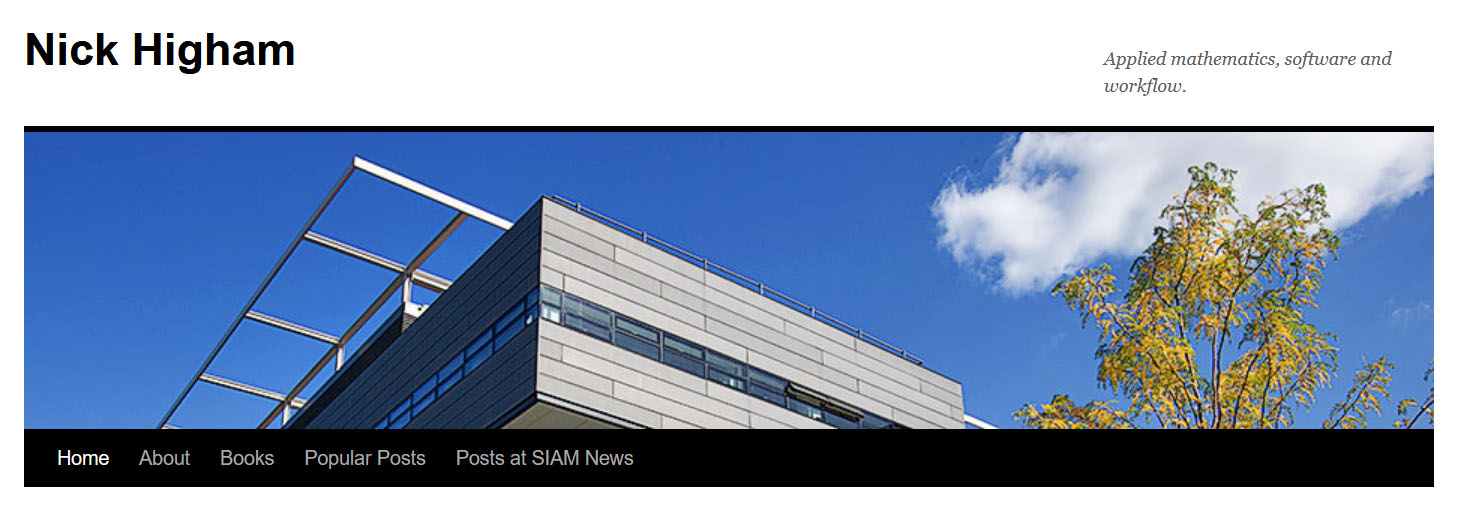
\includegraphics[width=.9\linewidth]{nickhighamwordpress.jpg}
\end{center}
\end{enumerate}
\end{document}